\titleformat{\chapter}{}{}{0em}{\bf\LARGE\thechapter.~}
\chapter{A probléma megoldása, részfeladatok}

\section{A feladat}

\begin{itemize}
  \item{két azonos számú affin függvénnyel definiált iterált függvényrendszer által generált fraktál egymásba transzformálása úgy, hogy a transzformáció során a generált fraktálok box-dimenziójának valamilyen alsó becslést tudjunk adni.}
  \item{a definiáló háromszögek csúcsai között olyan folytonos görbék keresése (valamilyen genetikus függvénnyel), amelyek mentén a lépésenként generált fraktálok box-dimenziója egy alsó korlát alá nem csökken.}
  \item{Apophysis-hez hasonló kezelőfelület kialakítása}
  \item{mentési lehetőség megvalósítása, a generált fraktálok animációja és a függvények szintjén egyaránt}
\end{itemize}

\section{Részfeladatok}
A probléma megoldására a következő részfeladatok lettek megfogalmazva:

\begin{itemize}
	\item {a matematikai háttér alapos ismerete és kidolgozása}
	\item {algoritmusok kidolgozása: (fraktálgenerálás, fraktál deformáció, box-dimenzió kiszámítása, genetikus algoritmus amely olyan folytonos görbéket keres amelyek mentén a lépésenként generált fraktálok box-dimenziója nem csökken egy alsó korlát alá)}
	\item {a kidolgozott algoritmusok implementációja Java nyelvbe}
	\item {dokumentáció készítése a program megvalósításáról és működéséről}
\end{itemize}

A feladat megoldása közben a legnagyobb kihívást a box-dimenzió becslése jelentette, a legtöbb időt az algoritmusok kidolgozása és implementálása vette igénybe. Különösen sok ráfordítást igényelt az n kontrolponttal rendelkező Basier görbék implementációja. Az implementálás Java nyelvben történt a JOGL függvénykönyvtár használatával.

\section{A munka végeredménye}
Egy olyan program, amely különböző fraktálok egybetranszformálását teszi lehetővé. A program képes háromszögek, valamint iterált függvényrendszerek segítségével fraktálokat kigenerálni, valamint ezeket egymásba transzformálni. Feltétel, hogy a két fraktált azonos számú affin függvény kell meghatározza.

\chapter{Alapfogalmak}

\section{Fraktál}
A legegyszerűbb, de nem feltétlenül pontos megközelítésben – „önhasonló”, végtelenül komplex geometriai alakzatok. Az önhasonlóság azt jelenti, hogy egy kisebb rész felnagyítva ugyanolyan struktúrát mutat, mint egy nagyobb rész. Az eredeti és talán legszélesebb körben elfogadott definíció, miszerint fraktálnak nevezünk egy geometriai alakzatot akkor, ha „induktív” dimenziója (Lebesgue-dimenziója) nem esik egybe (szigorúan kisebb) a Hausdorff-féle dimenziójával.

\section{Transzformáció}
A matematikában, elsősorban a geometriában transzformáció alatt egy halmaz önmagába való leképezéseit értjük. Speciális esetként a geometriai transzformációk olyan függvények, amelyek pontokhoz pontokat rendelnek hozzá, tehát értékkészletük és értelmezési tartományuk ponthalmaz.

\section{Affin transzformáció}
Az affin geometriában használt, illetve a lineáris algebra részeként is tárgyalható fogalom. Egy affin transzformáció során a transzformált koordináták az eredeti koordináták lineáris függvényeként állnak elő. Ide tartoznak a lineáris transzformációk és az eltolás is.
Iterált függvényrendszer, Iterated Function System(IFS) – A matematikában használt módszer, amellyel fraktálokat építenek fel. Ezek az IFS fraktálok mindig önhasonlóak. Az iterált függvényrendszerek a dinamikai rendszerek tanulmányozásában is használatosak. 

\section{Példa}
Legyen egy lineáris transzformáció, amely egy pontot leképez egy másik pontba. A transzformációt a  következőképpen definiáljuk:

$l_{1}(0,0)=(0,0);$ $l_{1}(1,0)=(\frac{1}{2},0);$ $l_{1}(0,1)=(0,\frac{1}{2});$

$f_{1}, f_{2}, f_{3}: \mathbb{R} \Rightarrow \mathbb{R}$ Három pont által meghatározott affin transzformációk. \\
$f_{1}=l_{1}+\vec{v};$

Az $f_{1}$ egy affin transzformáció amit úgy kapunk meg, hogy egy lineáris transzformációt eltolunk egy $\vec{v}$ vektorral. Ebben az esetben a $\vec{v}=(0,0);$

\newpage

Grafikusan a következőt jelenti:

\begin{figure}[H]
	\centering	
	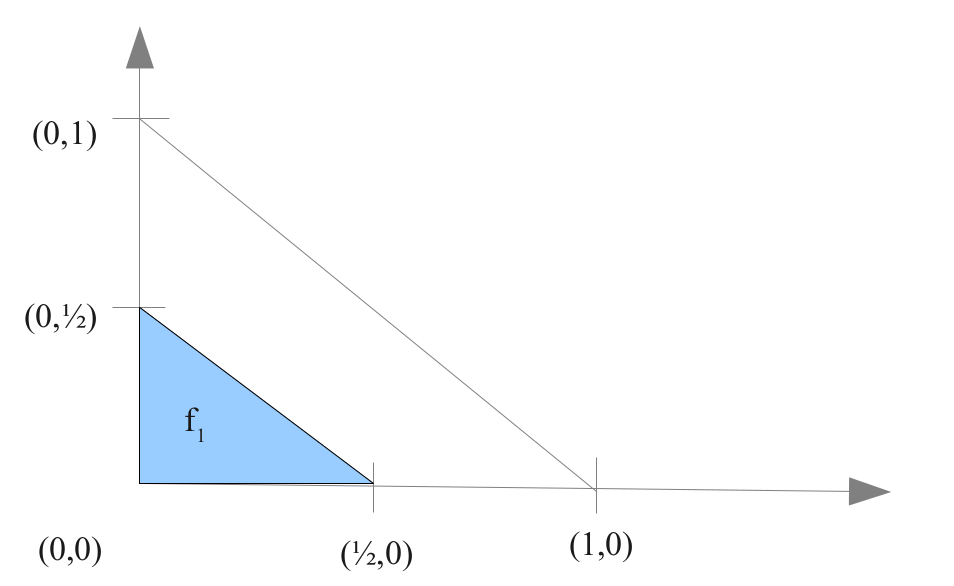
\includegraphics[scale=0.35]{Images/Grafikon1}
	\caption{Affin transzformáció}
\end{figure}

Az $f_{2}, f_{3}$ transzformációt az $f_1$-hez hasonlóképpen kapom meg:\\

$\{f_{2}(x,y)=f_{1}(x,y)+\vec{v}\}$ $\vec{v}=(\frac{1}{2},0)$; \\
\indent$\{f_{3}(x,y)=f_{1}(x,y)+\vec{u}\}$ $\vec{u}=(0,\frac{1}{2})$; \\

GRafikusan a következőképpen néz ki:

\begin{figure}[H]
	\centering	
	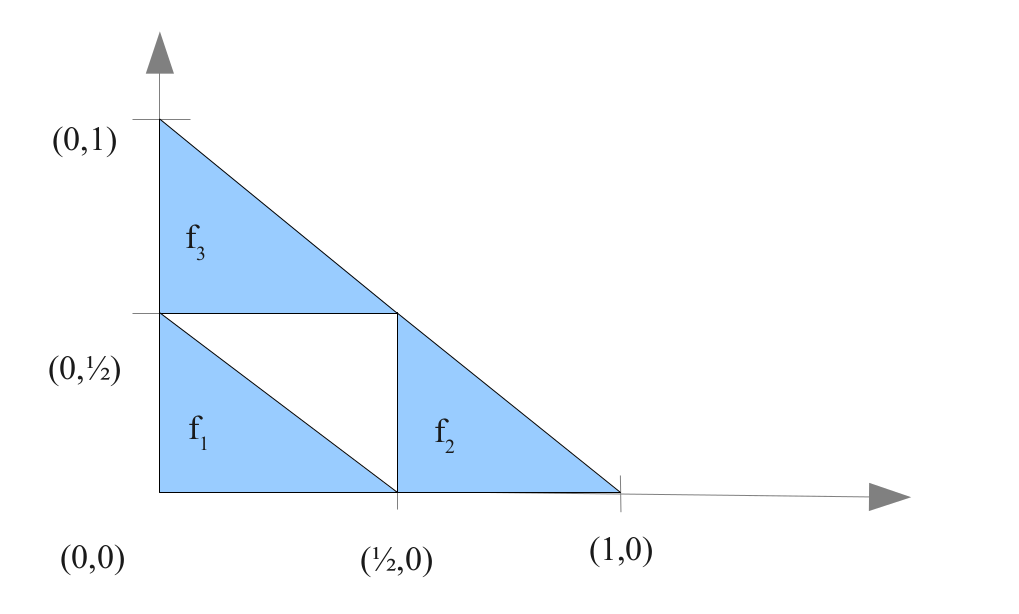
\includegraphics[scale=0.35]{Images/Grafikon2}
	\caption{Affin transzformációk}
\end{figure}


Ha a transzformációk segítségével megkapott kicsi háromszögekre újra és újra elvégezzük az előbbi
transzformációkat, akkor egy önhasonló struktúrát fogunk kapni. Nem szükséges minden lépésben(iterációban) elvégeznünk mind a három transzformációt, elég ha minden lépésben véletlenszerűen
kiválasztunk egyet. Esetünkben a Sierpinski háromszöget fogjuk megkapni.

\section{Fraktál deformáció}
Fraktál deformáció alatt azt a folyamatot értjük, amely egy meglevő fraktál képét, átképezi egy másik
fraktál képébe. Feltétel, hogy a két fraktál képét ugyanannyi pont határozza meg. A fraktál deformációt
a következő példa segítségével szemléltetjük:

Legyen $f_{1}, g_{1}: \mathbb{R} \Rightarrow \mathbb{R}$

\begin{figure}[H]
	\centering	
	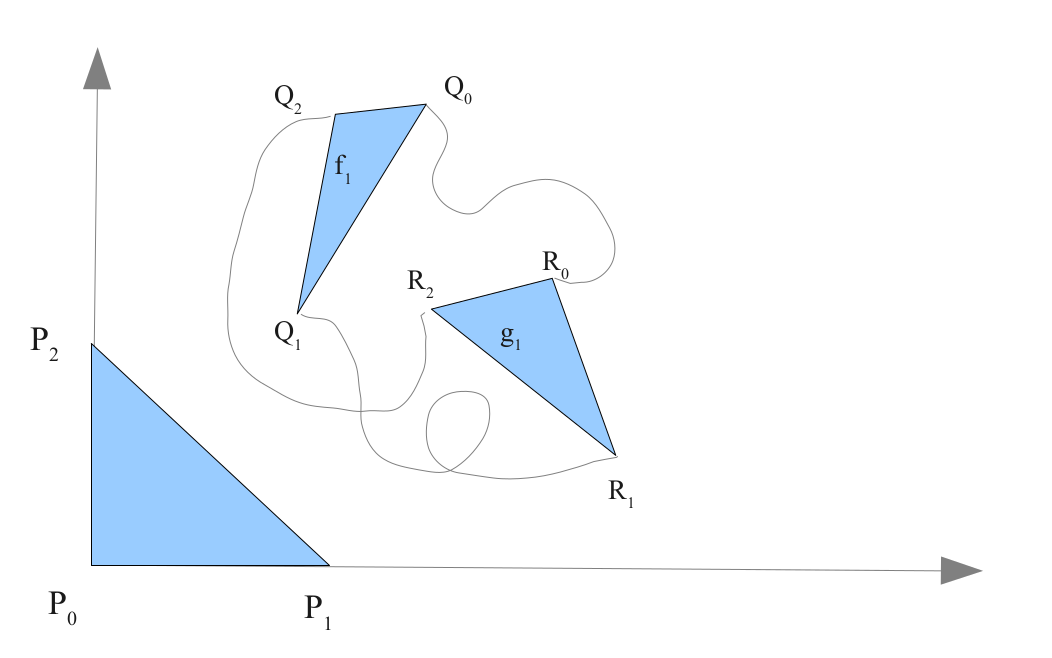
\includegraphics[scale=0.4]{Images/Grafikon3}
	\caption{Fraktál deformáció}
\end{figure}

Az $f_1{}$ transzformáció a $P_{0}, P_{1}, P_{2}$ pontokat viszi át a $Q_{0}, Q_{1}, Q_{2}$ pontokba, míg a $g_{1}$ transzformáció az $R_{0}, R_{1}, R_{2}$ pontokba. A fraktál deformáció esetén beszélhetünk egy $\gamma$ függvényről, amely valamilyen síkgörbe mentén, T idő alatt leképezi a $Q_{0}, Q_{1}, Q_{2}$ pontokat, az $R_{0}, R_{1}, R_{2}$ pontokra.\\

$\gamma: [0,1] \rightarrow \mathbb{R}^2$\\

Ez egy köztes $t_{1}$ időpillanatban, egy köztes $H_{t}$ fratkál képét tekinthetjük meg. Ezt a következő ábrán szemléltetjük.

\begin{figure}[H]
	\centering	
	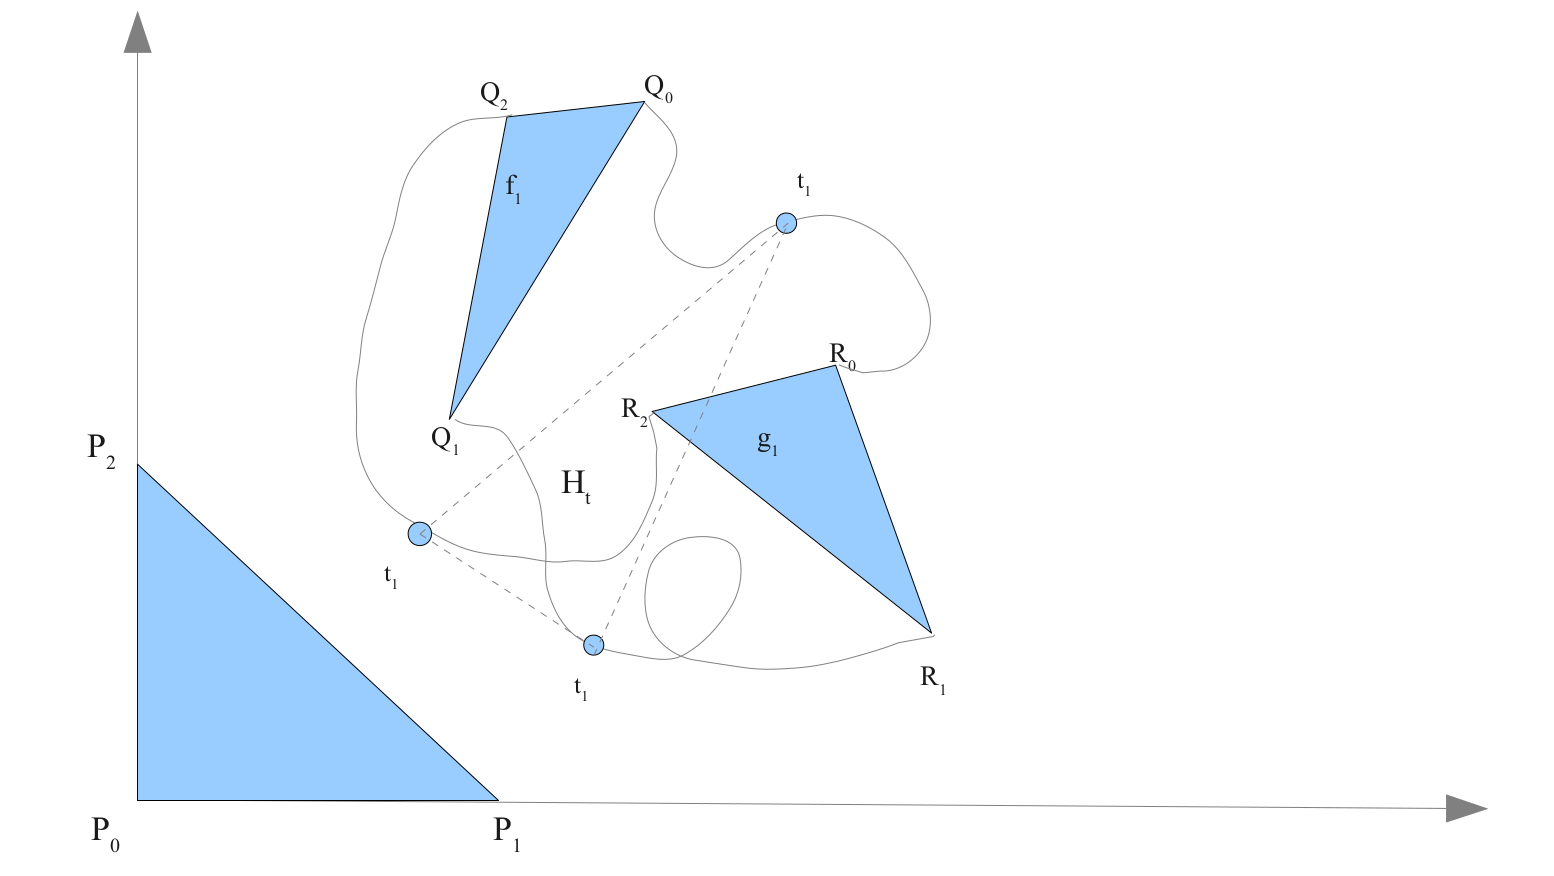
\includegraphics[scale=0.3]{Images/Figture4}
	\caption{Köztes állapot}	
\end{figure}	

\section{Box-dimenzió(Hausdorff-dimenzió,fraktáldimenzió)}

A fraktálgeometriában egy módszer, amellyel meg lehet határozni a fraktál dimenzióját egy Euklideszi
térben. A box-dimenzió kiszámításához, képzeljük el az adott fraktált egy egyenletesen elosztott
négyzethálóban elhelyezve és számoljuk meg, mennyi négyzetre van szükség, hogy befedje a teljes
halmazt. Minél sűrűbb ez a négyzetháló, annál jobban nő ez a szám.
Legyen $N(\varepsilon)$ a négyzetek száma, és $\varepsilon$ a négyzetek oldalainak hossza. Ekkor a következőképpen határozzuk meg a box-dimenziót:\\

$dim_{box}(S):=\lim\limits_{\varepsilon \rightarrow 0} \frac{lnN\varepsilon}{ln \frac{1}{\varepsilon}}$\\

„A fraktál olyan halmaz, aminek a Hausdorff-dimenziója nagyobb, mint a Lebesgue-dimenziója.” –
Mandelbrot.
Ahol a vonal Lebesgue-dimenziója egy, a felületé kettő, és így tovább. Ez alapján számítva a fraktálok
hossza vagy felszíne végtelen. A Hausdorff-dimenziót szemléletesen az adja, hogy hány példányra van
szükség az adott alakzatból ahhoz, hogy kirakjuk az alakzat egy nagyobb példányát. Ez csak szabályos
fraktál esetén alkalmazható.Például a Sierpinski-háromszög, ami önmagának három felére kicsinyített példányából áll, Hausdorff-dimenziója (box-dimenziója) $\frac{3}{2}\approx1,585$, míg Lebesgue-dimenziója 1.

\begin{figure}[H]
	\centering		
	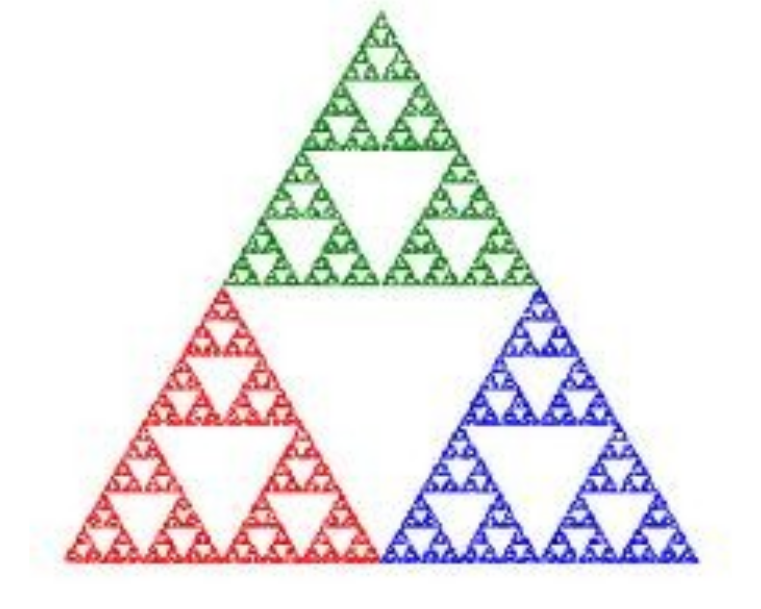
\includegraphics[scale=0.3]{Images/Sierpinski-triangle.png}
	\caption{Sierpinski-háromszög}
\end{figure}	

A Sierpinsi-szőnyeg box-dimenziója $\frac{ln8}{ln3}\approx1,89$

\begin{figure}[H]
	\centering	
	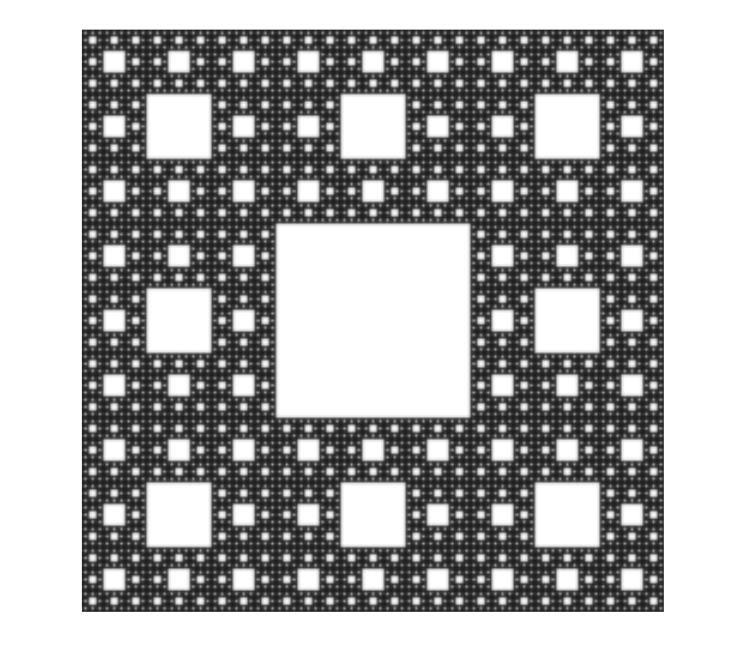
\includegraphics[scale=0.3]{Images/Sierpinski-szonyeg.png}
	\caption{Sierpinski-szőnyeg}	
\end{figure}

A Menger-szivacs box-dimenziója $\frac{ln20}{ln3}\approx2,73$

\begin{figure}[H]
	\centering
	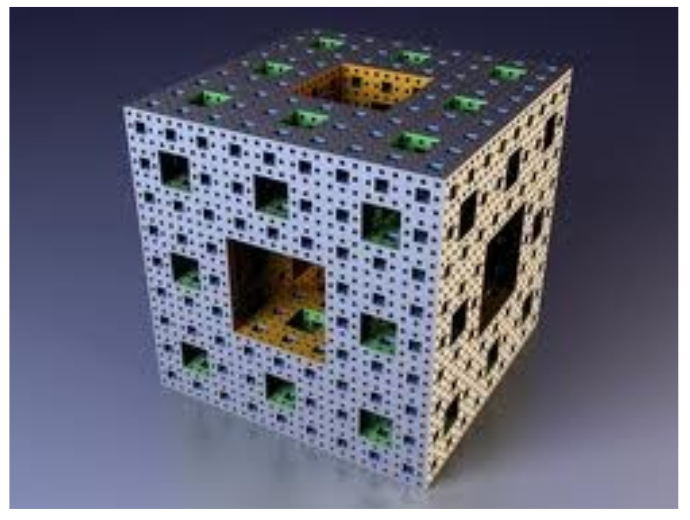
\includegraphics[scale=0.3]{Images/Menger-sponge.png}
	\caption{Menger sponge}	
\end{figure}

A Koch-hópehely box-dimenziója $\frac{ln4}{ln3}\approx1,26$

\begin{figure}[H]
	\centering
	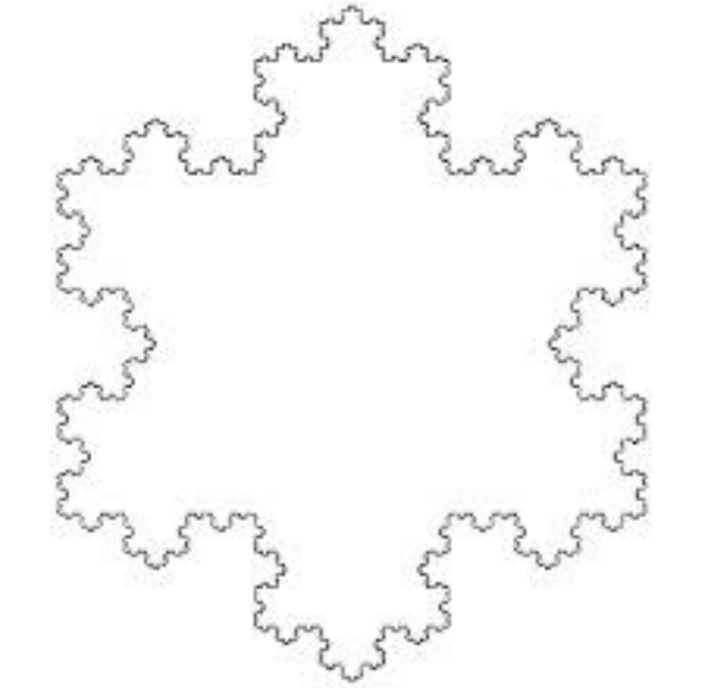
\includegraphics[scale=0.3]{Images/Kock-hopehely.png}
	\caption{Kock-hópehely}	
\end{figure}

\section{Genetikus algoritmusok}

Olyan keresési technikák egy osztálya, melyekkel optimumot vagy egy adott tulajdonságú elemet lehet keresni. A genetikus algoritmusok speciális evolúciós algoritmusok, a technikáikat az evolúcióbiológiából kölcsönözték. 
A genetikus algoritmusok sokfélék lehetnek, de az alábbi részeket mindig tartalmazzák: 

\subsection{Inicializáció}
A kezdeti populációt legegyszerűbb véletlenszerűen generálni. A populáció mérete a probléma természetétől függ, de leggyakrabban néhány száz vagy néhány ezer egyedből áll. Hagyományosan az egyedek a keresési téren egyenletesen oszlanak el, viszont egyes esetekben olyan részeken több egyedet generálnak, ahol sejthető az optimum. 

\subsection{Szaporítás (keresztezés)}
Egyedekből újabb egyedeket a kétoperandusú keresztezés (vagy rekombináció) művelettel, és az egyoperandusú mutáció művelettel lehet. Ezeket az operátorokat általában véletlenszerűen alkalmazzák. 

\subsection{Kiválasztás (szelekció)}
Az egyedek generálása után a kiválasztásra kerül sor. A kiválasztás lehet determinisztikus vagy stochasztikus. Az első esetben szigorúan az egy adott küszöbértéknél jobb állóképességű egyedek maradnak fenn, a stochasztikus kiválasztásnál a rosszabb állóképességű egyedek közül is néhány fennmarad. A stochasztikus megoldás népszerűbb, mert elkerülhető vele a lokális optimumhoz való konvergencia.

\subsection{Leállás}
A genetikus algoritmusok rendszerint addig futnak, amíg egy leállási feltétel nem teljesül. Gyakori leállási feltételek a következők: 

\begin{itemize}
	\item{Adott generációszám elérése.}
	\item{Ha a legjobb egyed állóképessége már nem javul jelentős mértékben egy-egy iterációval. }
\end{itemize}